% !TeX spellcheck = en_US
\documentclass{article}
\usepackage{pacco}
	\makeindex
\begin{document}
	\title{Probability theory notes}
	\author{Kotatsu}
	\date{\tiny TOALDO TI TROVERÒ E FARAI UNA BRUTTA FINE COL \textbf{CAZZO} CHE DIVENTI ORDINARIO}
	\maketitle
	\tableofcontents
\section{Basics of probability}
We start with the probability triplet: $(\Omega,\mathscr{H},\mathbbm{P})$ 
Here $\Omega$ is the set of sample space, $\mathscr{H}$ is the $\sigma$-algebra built upon $\Omega$ and $\pr$ is the probability measure. Since $\pr$ is a measure, it will take values in $\R$. \\
We are interested in probability measure, which means:
\begin{itemize}
	\item $\pr$ is a \textbf{finite measure} and $\pr(\Omega)=1$;
	\item $\omega \in\Omega$ will be called \textbf{outcomes}.
\end{itemize}
So consider the example of the roll of the die. If we roll it, 
\[\Omega=\underbrace{\left\{1,2,3,4,5,6\right\}}_{\text{outcomes}}\]
And if we considere the elements $A\in\mathscr{H}$ (which will be subsets of $\Omega$) will be called \textbf{events}.\par We want to quantify the possibility that the event $A$ occurs: we want to measure, through $\pr$, the set $A$: from a measure theory point of view, it's only sets in the $\sigma$-algebra. \\The probability measure has the following properties:
\begin{itemize}
	\item $\pr(\Omega)=1,\quad\pr(\emptyset)=0$
	\item \textbf{monotonicity of $\pr$}: take 2 events $H,K\in\mathscr{H}$ such that $H\subset K$. Then $\pr(H)\leqslant\pr(K)$\footnote{note that the notation is loose since we have proper subset on one side and leq on the other side. But this is not much of a problem, since i will kill myself very soon.}.
	\item \textbf{finite additivity}: take $H,K\in\mathscr{H}$ such that $H\cap K=\emptyset$. The $\pr(H\cup K)=\pr(H)+\pr(K)$;
	\item \textbf{countable additivity}: this requires that we consider collection of events. We denote them in this way:
	\[\left(H_n\right)_{n\in\N}\subset\mathscr{H}\] with $\N=\{0,1,2,3,\ldots\}$ and $\N^\star=\{1,2,3,4,\ldots\}$ such that they are disjoint pairwise (except identical pairs). Then
	\[\pr\left(\bigcup_nH_n\right)=\sum_n\pr\left(H_n\right)\]
	\item \textbf{Boole inequality (sub-additivity)}: if we have a collection $\left(H_n\right)_{n\in\N}\subset\mathscr{H}$ (not necessarily disjoint) then $$\pr\left(\bigcup_nH_n\right)\leqslant\sum_n\pr\left(H_n\right)$$ 
	\item \textbf{sequential continuity}: consider the sequence $\left(H_n\right)_{n\in\N}\subset\mathscr{H}$ such that $H_n\nearrow H\in\mathscr{H}$ ($H_n$ is an increasing sequence of numbers that has $H$ as limit) then $\pr(H_n)\nearrow\pr(H)$. Moreover, if $\left(F_n\right)_{n\in\N}\subset\mathscr{H}$ such that $F_n\searrow F\in\mathscr{H}$ then $\pr(F_n)\searrow\pr(F)$. The second property is actually true because $\pr$ is finite (it is not true for infinite measures). 
\end{itemize}
In measure theory we encounter the concept of \textbf{negligible sets}: these are sets of measure zero or non measurable sets included in measure zero sets. In probability theory, sets are \textbf{events}: so we have negligible events (events with probability 0 or non measurable events included in events with probability 0). Analogously, in measure theory a property which holds \textbf{almost everywhere} is allowed not to hold on negligible sets. In probability theory a property which holds \textbf{almost surely} is allowed not to hold on negligible events.
We also have, in measure theory, \textit{measurable functions} that in probability theory are \textbf{random variables}.
\subsection{Random variables}
Consider a measurable space $(E,\mathscr{E})$. 
\begin{definition}
	A mapping $X:\Omega\rightarrow E$ is called \enf{random variable taking values in $E$} if $X$ is measurable relative to $\mathscr{H}$ and $\mathscr{E}$.
\end{definition}
What does it mean\footnote{who asked}? The inverse image of the set $A$ through $X$ ($X^{-1}A$) with $A\in \mathscr{E}$ is actually the set of the $\omega$s such that $X(\omega)$ arrives to $A$. So
\[X^{-1}A=\left\{\omega\in\Omega:X(\omega)\in A\right\}=\left\{X\in A\right\}\] so that $X^{-1}A$ is an event for all $A$ in $\mathscr{E}$.
\begin{figure}[H]
	\centering
	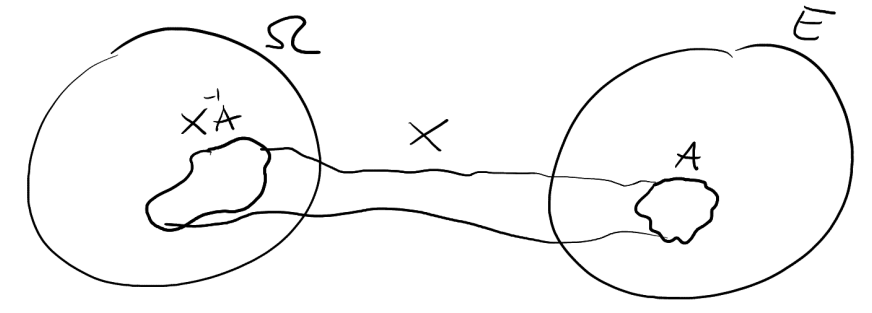
\includegraphics[width=0.7\linewidth]{screenshot001}
	\caption{this is an early reminder of the fact that I will take my own life very soon.}
	\label{fig:screenshot001}
\end{figure}
So if $X^{-1}A$ is measurable by $\pr$ then it is in $\mathscr{H}$: otherwise it is not in $\mathscr{H}$. So \[\pr(X^{-1}A)=\pr\left(\left\{\omega\in\Omega:X(\omega)\in A\right\}\right).\] The message is that I am interested/able to evaluate $\pr$ over the set only if what I am evaluating is indeed an event (which means: it belongs to $\mathscr{H}$\footnote{il lettore più arguto avrà notato che, a questo punto, il dio è ormai irrimediabilmente cane.}). If something is not in $\mathscr{H}$ get it off my fucking face man and kill yourself NOW\footnote{
		
\includegraphics[width=0.05\linewidth]{screenshot002}
}. This is the only restriction for a random variable. $E$ can be whatever we need it to be: a graph, a tree, your mom being absolutely \censor{torn apart} by me. But most of the times, we have $E=\R$ or $E=\R^d$ with respectively $\mathscr{E}=\mathscr{B}\footnote{Borel $\sigma$-algebra}(\R)=\mathscr{B}_\R$ and $\mathscr{B}_{\R^d}$.
\begin{remark}
	The simplest random variables are indicator functions of events.
	Example: take $H\in\mathscr{H}$. Define the function
	\begin{align*}
		\indi_H&:\Omega\rightarrow\R\\
		\indi_H(\omega)&=\begin{cases}
			0 &\omega\not\in H\\
			1 &\omega\in H
		\end{cases}
	\end{align*}
\end{remark}
\begin{remark}
	A random variable is said to be \enf{simple} if it takes only finitely many values in $\R^d$.
\end{remark}
\begin{remark}
	A random variable is said to be \enf{discrete} if it takes only countably many values.
\end{remark}
\begin{definition}
	\enf{Distribution of a random variable}. Let $X$ be a random variable taking values in $(E,\mathscr{E})$ and let $\mu$ be the image of $\pr$ under $X$, that is,
	\[\mu(A)=\pr(X^{-1}A)=\pr(X\in A)=\pr\circ X^{-1}(A)\footnote{you would know this if you knew fucking measure theory I guess},\;A\in\mathscr{E}.\] Then $\mu$ is a probability measyre on $(E,\mathscr{E})$ and it is called \textbf{distribution of X}.
\end{definition}
So we map, by means of $X$, sets belonging to $\mathscr{E}$ into $\mathscr{H}$ and then evaluates this sets by means of the measure $\pr$. This is what we mean when we say that distributions are ultimately built with the probability measure and the random variable. Distribution is itself a measure!
\begin{remark}
	You should remember (LOL) that when we want to specify a measure on a $\sigma$-algebra, it's enough to do it on a \textit{p-system}\footnote{a p-system is a simpler object than a $\sigma$-algebra: it is simply a collection of sets closed under intersection} generating that $\sigma$ algebra: by means of the monotone class theorem we are then able to extend the measure to the $\sigma$-algebra. \\
	This means that to specity $\mu$ it is enough to specify it on a \textit{p-system} which generates $\mathscr{E}$. For example, consider $E=\overline{\R}, \mathscr{E}=\mathscr{B}_{\overline{\R}}$. Consider the collection of sets $[-\infty,x],\;x\in\R$ which is of course a p-system because it is closed under intersection. Moreover, this shit generates the Borel sigma algebra on $\overline{\R}$. \\If we want to define a distribution, that is a measure, it is enough to define it on this p-system. Imagine that we apply our distribution measure to one set of this p-system
	\[c(x)\footnote{because it is a function of $x$}=\mu\left([-\infty,x]\right)=\pr(X\leq x),\qquad x\in\R\] by the monotone class theorem. So we have now specified the measure on the p-system. The part $\pr(X\leq x)$ reminds us of the undergraduate times\footnote{I already wanted to kill myself at that time.}: it is a distribution function! This is what our professor did implicitly to avoid using measure theory\footnote{I have noticed that my life has not benefited in ANY form since I have been introduced to measure theory.}.
\end{remark}
\subsection{Functions of random variables}
Consider $X$, a random variable taking values in $(E,\mathscr{E})$ and consider further a measurable space $(F,\mathscr{F})$. Let $f:E\rightarrow F$ be a measurable function relative to $\mathscr{E}$ and $\mathscr{F}$\footnote{This basically means that this bitch won't do anything evil. The whole point of measure theory, $\sigma$ algebras and all other shit is to ensure everything behaves.}. This function should me measurable by means of $\pr$, otherwise we couldn't do anything useful with it. Consider the composition
\[Y=f\circ X\qquad\text{such that}\;Y(\omega)=f\circ X(\omega)=f\big(X(\omega)\big),\;\omega\in\Omega.\]
This composition is a random variable taking values in $(F,\mathscr{F})$ which comes from the fact that measurable functions of measurable functions are still measurable. 
\begin{definition}
	Consider two random variables $X,Y$ taking values in $(E,\mathscr{E})$ and $(F,\mathscr{F})$ respectively. Consider the pair
	\[Z=(X,Y):\Omega\rightarrow E\times F.\]
	Why would we want to call it $Z$? It's because, beside being a random vector, it is in turn a random variable:
	\[Z(\omega)=(X(\omega),Y(\omega)).\]
	Since $E\times F$ is a product space, we should attach it the product $\sigma$-algebra. So $Z$ is a random variable taking values in $E\times F$. 
\end{definition}
Note that the product space $E\times F$ is endowed with the \sa $\mathscr{E}\otimes\mathscr{F}$, that is the product \sa generated by the collection of all possible rectangles between $E$ and $F$. We frequently have to look to special cases like random vectors that must take values in measurable spaces for them to make sense. This measurable space is naturally generated by the product \sa (but it may be generated by other $\sigma$-algebras\footnote{Repeatedly inflicting painful kicks on my gonads.}!).
\begin{definition}
	We call \enf{joint distribution} of $X$ and $Y$ the distribution of $Z$. 
\end{definition}
This is interesting, since we know that this variable has the specific structure of a random vector: we identify the distribution of this vector as the joint distribution of its two coordinates\footnote{it eludes me how anyone could find this interesting. We have to think about the whole vector as being distributed like its components separately}. 
\begin{remark}
	The product \sa $\mathscr{E}\otimes\mathscr{F}$ is generated by the p-system of measurable rectangles.
\end{remark}
On the product space, it is enough to only specify it on this p-system.\par
Let denote with $\pi$ the joint distribution of $X,y$. It is sufficient to specify
\[\pi(A\times B)=\pr(X\in A, Y\in B)\qquad\every  A\in\mathscr{E},B\in\mathscr{F}.\]
We exploited the measurability of $X$ and $Y$
\begin{definition}
	Given the joint distribution $\pi$, consider sets $A\in\mathscr{E},B\in\mathscr{F}$. Then we call \enf{marginal distribution of $X$}
	\[\pr(X\in A)=\pi(A\times F)\qquad\;\every  A\in\mathscr{E}\]
	and we call \enf{marginal distribution of $Y$}
	\[\pr(Y\in B)=\pi(E\times B)\qquad\;\every  B\in\mathscr{F}.\]
\end{definition}
We call it distribution because it is actually a measure! So we can call it with the notation of measure
	\[\mu(A)=\pr(X\in A)=\pi(A\times F)\qquad\;\every  A\in\mathscr{E}\] and \[\nu(B)=\pr(Y\in B)=\pi(E\times B)\qquad\;\every  B\in\mathscr{F}.\]This actually means that the second coordinate is fixed in being the \underline{whole space} $F$. Think about integrating the second coordinate along the real line when doing marginal distributions... this is the same thing here.\\
Now that we have joint and marginal distributions, what is the next step\footnote{Committing the deed, methinks.}?
\begin{definition}
	Let $X,Y$ be \rv s taking values in $(E,\mathscr{E})$ and $(F,\mathscr{F})$ respectively and let $\mu$ and $\nu$ be their respective distributions. Then $X$ and $Y$ are said to be \enf{independent} if their joint distribution is the product measure formed by their marginals.
	\[\pr(X\in A,Y\in B)=\pr(X\in A)\pr(Y\in B)\qquad\every  A\in \mathscr{E},B\in\mathscr{F}.\]
	This also means that 
	\[\pi=\mu\nu\]
\end{definition}
Here the marginals do not interact with each other. This is true for two random variables and we need\footnote{No.} something more general.
\begin{definition}
Let $(X_1,X_2,\ldots,X_n)$ be a finite collection of random variables. The collection is said to be an \enf{independency} if the distribution of $(X_1,X_2,\ldots,X_n)$ is the product of $\mu_1,\mu_2,\ldots,\mu_n$ where $\mu_i$ is the distribution of $X_i$, for $i=1,\ldots,n$.
\end{definition}
Cynlar is stupid I wish him dead to be frank for this independecy shit. Independecy is not even an english word. What the fuck? Anyway, what about infinite collections?
\begin{definition}
	Let $(X_n)_{_n}$ be an infinite collection of \rv s. It is said to be an \enf{independency} if every finite sub-collection of it is an independecy.
\end{definition}
We now turn to stochastic processes\footnote{Please no.}! But first...
\subsection{Infinite product spaces}
Let $T$ be an arbitrary (countable or uncountable) set. We will think about this set as an "index" set. For each $t\in T$ consider the measurable $(E_t,\mathscr{E}_t)$. So we have a space for each index (plenty of measurable spaces hanging around). Consider a point $x_t$ in $E_t$ for each $t\in T$. The collection\footnote{We could consider it a function of $t$ but that wouldn't be exactly correct since each $t$ has a different measurable space. We may have the same space but it's not true in general... I am thrilled to say the least.} $(x_t)_{_{t\in T}}$. If  $(E_t,\mathscr{E}_t)=(E,\mathscr{E})$ then $(x_t)_{_{t\in T}}$ is actually a function of $T$ taking values on $(E,\mathscr{E})$. \\
The set $F$ of all possible functions $x=(x_t)_{_{t\in T}}$ is called the \enf{product space}$\left((E_t\mathscr{E}_t)\right)_{_{t\in T}}$.\\ This is the natural generalization of what we do when we construct product spaces, albeit with a different notation. Usually $F$ is denoted by $X_{t\in T}E_t$. But we know we also need a \sa...\\
A \enf{rectange} in $F$ is a subset of the form
\[\{x\in F:x_t\in A_t \;\every t\in T\}\]
Where $A_t$ differs from $E_t$ for only a finite number of $t$.
\subsection{Stochastic processes}
\end{document}